% !Mode:: "TeX:UTF-8"	% read in as utf8 file.
\chapter{The Linear Tetrahedron}

\section*{Introduction}
This Chapter covers the formulation and implementation of the simplest solid element: the four-node tetrahedron. This is also called the linear tetrahedron since its shape functions are linear polynomials. Within a programming context, the name is often abbreviated to Tet4. We start with this particular element for two reasons: its geometry is the simplest one in three space dimensions, and no numerical integration is needed to construct element equations.

\section{The Linear Tetrahedron}
The linear tetrahedron, shown in figure \ref{fig:tet4_linearTetrahedron}(a), is often shunned for stress analysis because of if its poor performance. Its main value in structural and solid mechanics is educational: it serves as a vehicle to introduce the basic steps of formulation of 3D solid elements, particularly as regards use of natural coordinate systems, node numbering conventions and computational ingredients. It should be noted that 3D visualization is notoriously more difficult than 2D, so we need to proceed somewhat slowly here.

\begin{figure}[h]
\centering
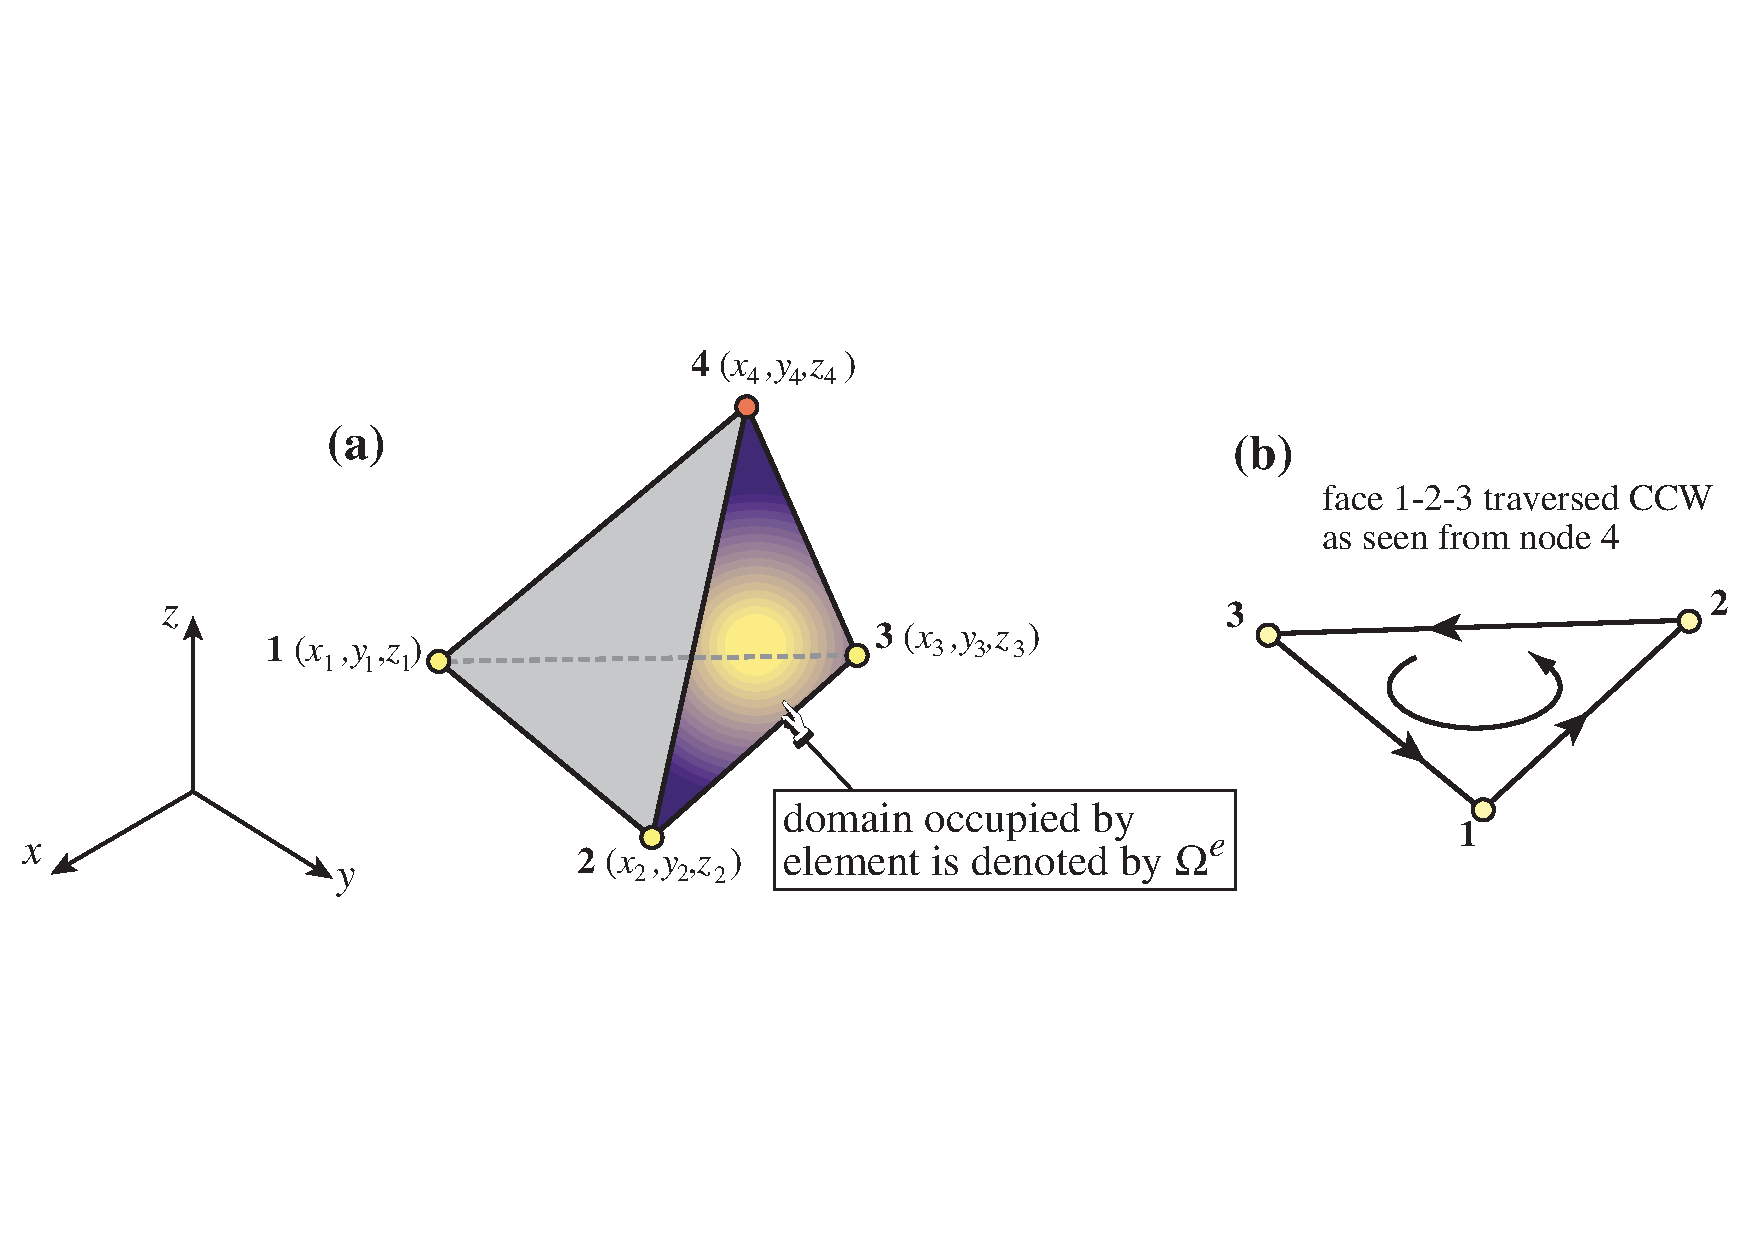
\includegraphics[width=0.7\linewidth]{figure/linearTetrahedron}
\caption{The four node tetrahedron element, also called the linear tetrahedron, or Tet4 in programming context: (a) element picture; (b) corner node numbering convention}
\label{fig:tet4_linearTetrahedron}
\end{figure}

\subsection{Tetrahedron Geometry}
We begin by placing the undeformed elastic object in a coordinate system, and denote by $ \Omega $ the volumetric domain occupied by the object. This domain will be referred as the \textit{reference (or undeformed) configuration}, and we follow the convention that capital letters $ \vec{X} \in \Omega $ are used when referring to individual material points in this underformed shape. Note that the precise position and orientation of the underformed elastic body within the reference space is not important and can be chosen at will, as long as the shape of the object corresponds to a rest configuration.

When the object undergoes deformation, every material point $ \vec{X} $ is being displaced to a new \textit{deformed} location which is, by convention, denoted by a lowercase variable $ \vec{x} $. 

Figure \ref{fig:tet4_linearTetrahedron} shows a typical four-node tetrahedron. Its geometry is fully defined by giving the position of the four corner nodes with respect to the global RCC system $ {X,Y,Z} $:

\begin{equation}
X_i, \quad Y_i, \quad Z_i \quad (i=1,2,3,4)
\end{equation}

We will often use the abbreviations for corner coordinate differences:

\begin{equation}
X_{ij}=X_i-X_j, \quad Y_{ij}=Y_i-Y_j, \quad Z_{ij}=Z_i-Z_j, \quad i,j=1,...,4
\end{equation}

The four corners are assumed not to be coplanar. The element has six sides (also known as edges) and four faces. Sides are straight because they are defined by two corner points. Faces are planar because they are defined by three corner points. At each corner three sides and three faces meet.

The domain occupied by the tetrahedron is denoted by $ \Omega^e $. See figure \ref{fig:tet4_linearTetrahedron}.

The volume measure of the tetrahedron is denoted by $ V $, which should not be confused with the domain identifier $ \Omega $ or $ \Omega^e $. The volume is given by the following determinant in terms of the corner coordinate values:

\begin{equation} \label{eq: tet4_volume}
\begin{split}
V &= \int_{\Omega^e} d\Omega^e  = \dfrac{1}{6} \det \begin{bmatrix}
1 & 1 & 1 & 1\\
X_1 & X_2 & X_3 & X_4\\
Y_1 & Y_2 & Y_3 & Y_4\\
Z_1 & Z_2 & Z_3 & Z_4
\end{bmatrix} = \dfrac{1}{6} \det (\mathbf{J}) = \dfrac{1}{6} J \\
&= \dfrac{X_{21}(Y_{23}Z_{34}-Y_{34}Z_{23})+X_{32}(Y_{34}Z_{12}-Y_{12}Z_{34})+X_{43}(Y_{12}Z_{23}-Y_{23}Z_{12})}{6} 
\end{split}
\end{equation}

The above displayed matrix (without the $ 1/6 $ factor) is called the \textit{Jacobian matrix} $ \mathbf{J} $ and its determinant the \textit{Jacobian determinant} $ J $ . Note that $ J $ is a signed quantity, and so is $ V = J/6 $. We will always assume that $ V $ is positive. This can be insured if the nodes are not coplanar, and are appropriately numbered. A numbering rule that achieves this goal is as follows:

\begin{enumerate}[I]
\item Pick a corner (any corner) as initial one. In Figure \ref{fig:tet4_linearTetrahedron}(a) this is that numbered 1.
\item Pick a face to contain the first three corners. The opposite corner will be numbered 4.
\item Number those three corners in a \textit{counterclockwise} sense when looking at the face from the opposite one. See Figure \ref{fig:tet4_linearTetrahedron}(b).
\end{enumerate}

Should the volume computed by \ref{eq: tet4_volume} be zero, this indicates that the four corner points are coplanar. This case should be flagged as an error.

\subsection{Coordinate Transformations}
Quantities that are intrinsically linked to the element geometry (e.g., shape functions) are best expressed in tetrahedron coordinates. On the other hand, quantities such as displacement, strain and stress components are expressed in the Cartesian system $ {x,y,z} $. Ergo, we need transformation equations to pass from one coordinate system to the other. The shape functions for linear tetrahedrons are: (one material point $ (X,Y,Z) $ inside a tetrahedron $ (X1,Y1,Z1),(X2,Y2,Z2),(X3,Y3,Z3),(X4,Y4,Z4) $ )

\begin{align*}
X(r,s,t) &= \Phi_1(r,s,t)X_1 + \Phi_2(r,s,t)X_2 + \Phi_3(r,s,t)X_3 + \Phi_4(r,s,t)X_4\\
Y(r,s,t) &= \Phi_1(r,s,t)Y_1 + \Phi_2(r,s,t)Y_2 + \Phi_3(r,s,t)Y_3 + \Phi_4(r,s,t)Y_4 \\
Z(r,s,t) &= \Phi_1(r,s,t)Z_1 + \Phi_2(r,s,t)Z_2 + \Phi_3(r,s,t)Z_3 + \Phi_4(r,s,t)Z_4
\end{align*}

for coordinates and:

\begin{align*}
u(r,s,t) &= \Phi_1(r,s,t)u_1 + \Phi_2(r,s,t)u_2 + \Phi_3(r,s,t)u_3 + \Phi_4(r,s,t)X_4u_4 \\
v(r,s,t) &= \Phi_1(r,s,t)v_1 + \Phi_2(r,s,t)v_2 + \Phi_3(r,s,t)v_3 + \Phi_4(r,s,t)X_4v_4 \\
w(r,s,t) &= \Phi_1(r,s,t)w_1 + \Phi_2(r,s,t)w_2 + \Phi_3(r,s,t)w_3 + \Phi_4(r,s,t)X_4w_4
\end{align*}

for the displacements.

Prepending the sum-of-tetrahedral-coordinates identity as first row we build the matrix relation:

\begin{equation} \label{eq: tet4_jacobian matrix}
\begin{bmatrix}
1 \\
X \\
Y \\
Z
\end{bmatrix} = \begin{bmatrix}
1 & 1 & 1 & 1 \\
X_1 & X_2 & X_3 & X_4 \\
Y_1 & Y_2 & Y_3 & Y_4 \\
Z_1 & Z_2 & Z_3 & Z_4
\end{bmatrix} \begin{bmatrix}
\Phi_1(r,s,t)\\
\Phi_2(r,s,t)\\
\Phi_3(r,s,t)\\
\Phi_4(r,s,t)
\end{bmatrix}
\end{equation}

The above $ 4 \times 4 $ matrix is called \textit{Jacobian} matrix of the linear tetrahedron. Explicit inversion gives:

\begin{equation}
\begin{bmatrix}
\Phi_1(r,s,t)\\
\Phi_2(r,s,t)\\
\Phi_3(r,s,t)\\
\Phi_4(r,s,t)
\end{bmatrix} = \dfrac{1}{6V} \begin{bmatrix}
6V_{01} & Y_{42}Z_{32}-Y_{32}Z_{42} & X_{32}Z_42-X_{42}Z_{32} & X_{42}Y_{32}-X_{32}Y_{42} \\
6V_{02} & Y_{31}Z_{43}-Y_{34}Z_{13} & Z_{43}Z_{31}-X_{13}Z_{34} & X_{31}Y_{43}-X_{34}Y_{13}\\
6V_{03} & Y_{24}Z_{14}-Y_{14}Z_{24} & X_{14}Z_{24}-X_{24}Z_{14} & X_{24}Y_{14}-X_{14}Y_{24}\\
6V_{04} & Y_{13}Z_{21}-Y_{12}Z_{31} & X_{21}Z_{13}-X_{31}Z_{12} & X_{13}Y_{21}-X_{12}Y_{31}
\end{bmatrix} \begin{bmatrix}
1\\
X\\
Y\\
Z
\end{bmatrix}
\end{equation}

The first column entries are explicitly given by:

\begin{align*}
6V_{01} &= X_2(Y_3 Z_4- Y_4 Z_3) + X_3(Y_4 Z_2 - Y_2 Z_4) + X_4(Y_2 Z_3 - Y_3 Z_2)\\
6V_{02} &= X_1(Y_4 Z_3 - Y_3 Z_4) + X_3(Y_1 Z_4 - Y_4 Z_1) + X_4(Y_3 Z_1 - Y_1 Z_3)\\
6V_{03} &= X_1(Y_2 Z_4 - Y_4 Z_2) + X_2(Y_4 Z_1 - Y_1 Z_4) + X_4(Y_1 Z_2 - Y_2 Z_1)\\
6V_{04} &= X_1(Y_3 Z_2 - Y_2 Z_3) + X_2(Y_1 Z_3 - Y_3 Z_1) + X_3(Y_2 Z_1 - Y_1 Z_2)
\end{align*}

These $ V_{0i} $ have the following geometric interpretation: signed volumes of the tetrahedra formed by the origin $ x=y=z=0 $ and faces 234, 341, 412 and 123, for $ i=1,2,3,4 $, respectively. That physical interpretation suggests the identity:

\begin{equation}
V = V_{01} + V_{02} + V_{03} + V_{04}
\end{equation}

To facilitate use of the summation convention to represent entries of the rightmost three columns in foregoing matrix using a more compact notation:

\begin{equation} \label{eq: tet4_inverse jacobian matrix}
\begin{bmatrix}
\Phi_1(r,s,t)\\
\Phi_2(r,s,t)\\
\Phi_3(r,s,t)\\
\Phi_4(r,s,t)
\end{bmatrix} = \dfrac{1}{6V} \begin{bmatrix}
6V_{01} & a_1 & b_1 & c_1 \\
6V_{02} & a_2 & b_2 & c_2\\
6V_{03} & a_3 & b_3 & c_3\\
6V_{04} & a_4 & b_4 & c_4
\end{bmatrix} \begin{bmatrix}
1\\
X\\
Y\\
Z
\end{bmatrix}
\end{equation}

\subsection{Partial Derivatives}
From eq. \ref{eq: tet4_jacobian matrix} and \ref{eq: tet4_inverse jacobian matrix} we can easily find the following relations that connect partial derivatives of Cartesian and tetrahedral coordinates:

\begin{align*}
\dfrac{\partial X}{\partial \Phi_i} = X_i, \quad \dfrac{\partial Y}{\partial \Phi_i} = Y_i, \quad \dfrac{\partial Z}{\partial \Phi_i} = Z_i, \quad i=1,2,3,4\\
6V\dfrac{\partial \Phi_i}{\partial X} = a_i, \quad 6V\dfrac{\partial \Phi_i}{\partial Y} = b_i, \quad 6V\dfrac{\partial \Phi_i}{\partial Z} = c_i, \quad i=1,2,3,4
\end{align*}

Partial derivatives of a function $ F(\Phi_1, \Phi_2, \Phi_3, \Phi_4) $ with respect to Cartesian coordinates follow the chain rule:

\begin{equation}\label{eq: tet4_partial differential rules}
\begin{split}
\dfrac{\partial F}{\partial X} &= \dfrac{\partial F}{\partial \Phi_i} \dfrac{\partial \Phi_i}{\partial X} = \dfrac{1}{6V} \left( \dfrac{\partial F}{\partial \Phi_1} a_1 + \dfrac{\partial F}{\partial \Phi_2} a_2 + \dfrac{\partial F}{\partial \Phi_3} a_3 + \dfrac{\partial F}{\partial \Phi_4} a_4\right) = \dfrac{a_i}{6V} \dfrac{\partial F}{\partial \Phi_i} \\
\dfrac{\partial F}{\partial Y} &= \dfrac{\partial F}{\partial \Phi_i} \dfrac{\partial \Phi_i}{\partial Y} = \dfrac{1}{6V} \left( \dfrac{\partial F}{\partial \Phi_1} b_1 + \dfrac{\partial F}{\partial \Phi_2} b_2 + \dfrac{\partial F}{\partial \Phi_3} b_3 + \dfrac{\partial F}{\partial \Phi_4} b_4\right) = \dfrac{b_i}{6V} \dfrac{\partial F}{\partial \Phi_i} \\
\dfrac{\partial F}{\partial Z} &= \dfrac{\partial F}{\partial \Phi_i} \dfrac{\partial \Phi_i}{\partial Z} = \dfrac{1}{6V} \left( \dfrac{\partial F}{\partial \Phi_1} c_1 + \dfrac{\partial F}{\partial \Phi_2} c_2 + \dfrac{\partial F}{\partial \Phi_3} c_3 + \dfrac{\partial F}{\partial \Phi_4} c_4\right) = \dfrac{c_i}{6V} \dfrac{\partial F}{\partial \Phi_i}
\end{split}
\end{equation}

\subsection{Displacement Interpolation}
The displacement field over the tetrahedron is defined by the three components $ u_x, u_y \mathrm{and} u_z $. These are linearly interpolated from their node values:

\begin{equation} \label{eq: tet4_displacement interpolation}
\vec{u} = \begin{bmatrix}
u_x\\
u_y\\
u_z
\end{bmatrix} = \begin{bmatrix}
u_{x1} & u_{x2} & u_{x3} & u_{x4}\\
u_{y1} & u_{y2} & u_{y3} & u_{y4}\\
u_{z1} & u_{z2} & u_{z3} & u_{z4}
\end{bmatrix} = \begin{bmatrix}
\Phi_1(r,s,t)\\
\Phi_2(r,s,t)\\
\Phi_3(r,s,t)\\
\Phi_4(r,s,t)
\end{bmatrix}
\end{equation}

The \textit{isoparametric definition} of the four-node tetrahedron as a displacement model:

\begin{equation}
\begin{bmatrix}
1\\
X\\
Y\\
Z\\
u_x\\
u_y\\
u_z
\end{bmatrix} = \begin{bmatrix}
1 & 1 & 1 & 1\\
X_1 & X_2 & X_3 & X_4\\
Y_1 & Y_2 & Y_3 & Y_4\\
Z_1 & Z_2 & Z_3 & Z_4\\
u_{x1} & u_{x2} & u_{x3} & u_{x4}\\
u_{y1} & u_{y2} & u_{y3} & u_{y4}\\
u_{z1} & u_{z2} & u_{z3} & u_{z4}
\end{bmatrix} \begin{bmatrix}
\Phi_1(r,s,t)\\
\Phi_2(r,s,t)\\
\Phi_3(r,s,t)\\
\Phi_4(r,s,t)
\end{bmatrix}
\end{equation}

The $ 12 \times 1 $ node displacement vector is configured node-wise as

\begin{equation}
\vec{u}^e = \begin{bmatrix}
u_{x1}\\
u_{y1}\\
u_{z1}\\
u_{x2}\\
u_{y2}\\
u_{z2}\\
\vdots\\
u_{z4}
\end{bmatrix} = \begin{bmatrix}
u_1\\
u_2\\
u_3\\
u_4
\end{bmatrix}
\end{equation}

\subsection{The Strain Field (geometrical equations)}
The \textbf{element} strain field is strongly connected to the displacements by the strain-displacement equations, which in indicial notation read:

\begin{equation}
e_{ij} = \dfrac{1}{2} ( u_{i,j} + u_{j,i})
\end{equation}

We translate this to matrix notation as follows. First, the six independent components of the stress tensor are arranged into a 6-component strain vector as follows:

\begin{equation} \label{eq: tet4_strain in vector form}
\mathbf{e} = \begin{bmatrix}
e_{11} & e_{22} & e_{33} & 2e_{12} & 2e_{23} & 2e_{31}
\end{bmatrix}^T = \begin{bmatrix}
e_{xx} & e_{yy} & e_{zz} & \gamma_{xy} & \gamma_{yz} & \gamma_{zy}
\end{bmatrix}^T
\end{equation}

The second expression shows the engineering notation for the shear strains. Second, displacement components $ u_1,u_2 \mathrm{and} u_3 $ are written as $ u_x, u_y \mathrm{and} u_z $, collected into a 3-vector and linked to the displacement field:

\begin{equation}
\mathbf{e} = \begin{bmatrix}
e_{xx}\\
e_{yy}\\
e_{zz}\\
2e_{xy}\\
2e_{yz}\\
2e_{zx}
\end{bmatrix} = \begin{bmatrix}
\dfrac{\partial}{\partial x} & 0 & 0\\
0 & \dfrac{\partial}{\partial y} & 0\\
0 & 0 & \dfrac{\partial}{\partial z}\\
\dfrac{\partial}{\partial y} & \dfrac{\partial}{\partial x} & 0\\
0 & \dfrac{\partial}{\partial z} & \dfrac{\partial}{\partial y}\\
\dfrac{\partial}{\partial z} & 0 & \dfrac{\partial}{\partial x}
\end{bmatrix}\begin{bmatrix}
u_x\\
u_y\\
u_z
\end{bmatrix} = \mathbf{D}\vec{\mathbf{u}}
\end{equation}

Combine this with eq. \ref{eq: tet4_displacement interpolation} and using the partial differentiation rules eq. \ref{eq: tet4_partial differential rules} we obtain the matrix relation between strains and nodal displacements:

\begin{equation}
\mathbf{e} = \mathbf{B} \mathbf{u}^e
\end{equation}

If the node displacements are arranged node-by-node, the matrix $ \mathbf{B} $ has the following configuration:

\setcounter{MaxMatrixCols}{20}
\begin{equation} \label{eq: tet4_matrix B}
\begin{split}
\mathbf{B} &= \dfrac{1}{6V} \begin{bmatrix}
a_1 & 0 & 0 & a_2 & 0 & 0 & a_3 & 0 & 0 & a_4 & 0 & 0\\
0 & b_1 & 0 & 0 & b_2 & 0 & 0 & b_3 & 0 & 0 & b_4 & 0\\
0 & 0 & c_1 & 0 & 0 & c_2 & 0 & 0 & c_3 & 0 & 0 & c_4\\
b_1 & a_1 & 0 & b_2 & a_2 & 0 & b_3 & a_3 & 0 & b_4 & a_4 & 0\\
0 & c_1 & b_1 & 0 & c_2 & b_2 & 0 & c_3 & b_3 & 0 & c_4 & b_4\\
c_1 & 0 & a_1 & c_2 & 0 & a_2 & c_3 & 0 & a_3 & c_4 & 0 & a_4
\end{bmatrix}\\
&= \dfrac{1}{6V}\begin{bmatrix}
B_1 & B_2 & B_3 & B_4
\end{bmatrix}
\end{split}
\end{equation}

Note that this matrix is constant over the element.

\subsection{The Stress Field}
The stress field is related to the strain field by the strong connection:

\begin{equation}
\sigma_{ij} = C_{ijkl} e_{kl}
\end{equation}

To convert this matrix notation we rearrange the 6 independent components to correspond to the strains \ref{eq: tet4_strain in vector form}:

\begin{equation} \label{eq: tet4_stress in vector form}
\mathbf{\sigma} = \begin{bmatrix}
\sigma_{11} & \sigma_{22} & \sigma_{33} & \sigma_{12} & \sigma_23 & \sigma_{31}
\end{bmatrix}^T = \begin{bmatrix}
\sigma_{xx} & \sigma_{yy} & \sigma_{zz} & \sigma_{xy} & \sigma_{yz} & \sigma_{zx}
\end{bmatrix}^T
\end{equation}

If the material is linearly elastic and no initial strains are considered, the constitutive equation may be compactly expressed as

\begin{equation} \label{eq: tet4_contitutive equation}
\mathbf{\sigma} = \mathbf{E}\mathbf{e}
\end{equation}

where the $ 6 \times 6 $ elasticity matrix $ E $ is symmetric. For a general anisotropic material the expanded form of \ref{eq: tet4_contitutive equation} is 

\begin{equation}
\begin{bmatrix}
\sigma_{xx}\\
\sigma_{yy}\\
\sigma_{zz}\\
\sigma_{xy}\\
\sigma_{yz}\\
\sigma_{zx}
\end{bmatrix} = \begin{bmatrix}
E_{11} & E_{12} & E_{13} & E_{14} & E_{15} & E_{16}\\
       & E_{22} & E_{23} & E_{24} & E_{25} & E_{26}\\
       &        & E_{33} & E_{34} & E_{35} & E_{36}\\
       &        &        & E_{44} & E_{45} & E_{46}\\
       &        &        &        & E_{55} & E_{56}\\
symm   &        &        &        &        & E_{66}
\end{bmatrix} \begin{bmatrix}
e_{xx}\\
e_{yy}\\
e_{zz}\\
2e_{xy}\\
2e_{yz}\\
2e_{zx}
\end{bmatrix}
\end{equation}

in which $ E_{ij} $ are constitutive moduli. If the material is isotropic, with elastic modulus $ E $ and Poisson's ratio $ v $, the foregoing relation simplifies to

\begin{equation}
\begin{bmatrix}
\sigma_{xx}\\
\sigma_{yy}\\
\sigma_{zz}\\
\sigma_{xy}\\
\sigma_{yz}\\
\sigma_{zx}
\end{bmatrix} = \dfrac{E}{(1+v)(1-2v)} \begin{bmatrix}
1-v & v & v & 0 & 0 & 0\\
v & 1-v & v & 0 & 0 & 0\\
v & v & 1-v & 0 & 0 & 0\\
0 & 0 & 0 & \dfrac{1}{2}-v & 0 & 0\\
0 & 0 & 0 & 0 & \dfrac{1}{2}-v & 0\\
0 & 0 & 0 & 0 & 0 & \dfrac{1}{2}-v
\end{bmatrix} \begin{bmatrix}
e_{xx}\\
e_{yy}\\
e_{zz}\\
2e_{xy}\\
2e_{yz}\\
2e_{zx}
\end{bmatrix}
\end{equation}

\subsection{The Element Stiffness Matrix}
Introducing $ \mathbf{e} = \mathbf{B} \mathbf{u} $ and $ \mathbf{\sigma} = \mathbf{C} \mathbf{e} $ into TPE functional restricted to the element volume and rendering the resulting algebraic form stationary with respect to the node displacements $ \mathbf{u}^e $ we get the usual expression for the element for the element stiffness matrix

\begin{equation}
\mathbf{K}^e = \int_{\Omega^e} \mathbf{B}^T \mathbf{C} \mathbf{B} d \Omega^e
\end{equation}

Assuming that elastic moduli do not vary over the element, the foregoing integrand is constant because matrix $ \mathbf{B} $ as given by eq. \ref{eq: tet4_matrix B} is constant. Since $ V = \int_{\Omega^e} d \Omega^e $ we get

\begin{equation}
\mathbf{K}^e = V \mathbf{B}^T \mathbf{C} \mathbf{B}
\end{equation}

This stiffness matrix $ 12 \times 12 $. It can be directly evaluated in closed form using the above expression or, equivalently, by a one-point (centroid) integration rule.

\fbox{I assume that $ \mathbf{K}_{ik}^e = V \mathbf{B}_i^T C_{ijkl} B_k, i,k = 1,2,3,4 $}

